% Figure from MATH 591 notes, section 4. Compile with the notes preamble.
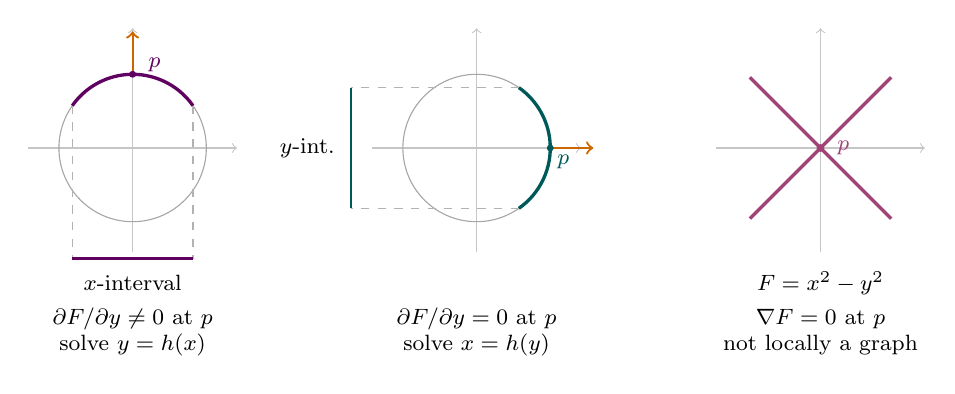
\begin{tikzpicture}[scale=0.78]
\foreach \dx in {0, 5.6, 11.2} {
  \draw[gray!45,->] (\dx-1.7,0) -- (\dx+1.7,0);
  \draw[gray!45,->] (\dx,-1.7) -- (\dx,1.95);
}
\draw[gray!70] (0,0) circle (1.2);
\draw[violet!75!black,very thick] (35:1.2) arc (35:145:1.2);
\draw[dashed,gray!60] (145:1.2) -- ({1.2*cos(145)},-1.8);
\draw[dashed,gray!60] (35:1.2) -- ({1.2*cos(35)},-1.8);
\draw[violet!75!black,thick] ({1.2*cos(145)},-1.8) -- ({1.2*cos(35)},-1.8);
\draw[orange!80!black,->,thick] (0,1.2) -- (0,1.9);
\fill[violet!75!black] (0,1.2) circle (1.6pt);
\node[violet!75!black,font=\footnotesize,anchor=west] at (0.1,1.36) {$p$};
\node[font=\footnotesize] at (0,-2.2) {$x$-interval};
\node[font=\footnotesize,align=center] at (0,-3.0) {$\partial F/\partial y\neq0$ at $p$\\ solve $y=h(x)$};
\draw[gray!70] (5.6,0) circle (1.2);
\draw[teal!70!black,very thick] ([shift={(5.6,0)}]-55:1.2) arc (-55:55:1.2);
\draw[dashed,gray!60] ([shift={(5.6,0)}]55:1.2) -- (3.55,{1.2*sin(55)});
\draw[dashed,gray!60] ([shift={(5.6,0)}]-55:1.2) -- (3.55,{-1.2*sin(55)});
\draw[teal!70!black,thick] (3.55,{-1.2*sin(55)}) -- (3.55,{1.2*sin(55)});
\draw[orange!80!black,->,thick] (6.8,0) -- (7.5,0);
\fill[teal!70!black] (6.8,0) circle (1.6pt);
\node[teal!70!black,font=\footnotesize,anchor=north west, inner sep=1.5pt] at (6.84,-0.04) {$p$};
\node[font=\footnotesize,anchor=east] at (3.45,0) {$y$-int.};
\node[font=\footnotesize,align=center] at (5.6,-3.0) {$\partial F/\partial y=0$ at $p$\\ solve $x=h(y)$};
\draw[magenta!60!black,very thick] (10.05,-1.15) -- (12.35,1.15);
\draw[magenta!60!black,very thick] (10.05,1.15) -- (12.35,-1.15);
\fill[magenta!60!black] (11.2,0) circle (1.8pt);
\node[magenta!60!black,font=\footnotesize,anchor=west, inner sep=1pt] at (11.42,0) {$p$};
\node[font=\footnotesize] at (11.2,-2.2) {$F=x^2-y^2$};
\node[font=\footnotesize,align=center] at (11.2,-3.0) {$\nabla F=0$ at $p$\\ not locally a graph};
\end{tikzpicture}
